\documentclass[a4paper,11pt,UTF8]{article}
\usepackage{ctex}
\usepackage{amsmath,amsthm,amssymb,amsfonts}
\usepackage{amsmath}
\usepackage[a4paper]{geometry}
\usepackage{graphicx}
\usepackage{microtype}
\usepackage{subfigure}
\usepackage{booktabs}
\usepackage[colorlinks=false, pdfborder={0 0 0}]{hyperref}
\usepackage{cleveref}
\usepackage{esint} 
\usepackage{graphicx}
\usepackage{ragged2e}
\usepackage{pifont}
\usepackage{extarrows}
\usepackage{mathptmx}
\usepackage{float}
\usepackage{caption}
\captionsetup[figure]{name={Figure}}
%opening
\title{华工激光:激光技术与中国特色社会主义思想的实践体验}
\author{谢悦晋}
\date{}
\begin{document}
\maketitle
\section{调查背景及意义}
习近平总书记在中国科学院第二十次院士大会、中国工程院第十五次院士大会和中国科协第十次全国代表大会上的指出:科技立则民族立,科技强则国家强。在党中央坚强领导下,在全国科技界和社会各界共同努力下,我国科技实力正在从量的积累迈向质的飞跃、从点的突破迈向系统能力提升,科技创新取得新的历史性成就。实践证明,我国自主创新事业是大有可为的,我国广大科技工作者是大有作为的。我们完全有基础、有底气、有信心、有能力抓住新一轮科技革命和产业变革的机遇,乘势而上,大展宏图。华工激光是我们华中大孕育的企业,作为高新技术公司的典型代表,华工激光在华中工学院的孕育下形成了自己的激光技术体系,代表了国家竞争力,具备了国际竞争力,成为世界级的激光设备提供商。同时,华工激光深刻贯彻了习近平总书记对于科技强国的要求,他们以创新为自己的核心价值观,在创新的过程中提倡竞争精神、形成竞争机制,提高核心竞争力段。

为了了解华工激光是怎样走出这样一条科技自强道路,电信学院2022级提高2201班团支部组织参观了华工激光的科技馆。
\section{调查方式}
参观前首先查阅了华工激光的相关资料,在基本了解华工激光的概括后前往公司实地考察,通过跟随讲解员讲解的方式了解华工激光的技术发展。
\section{调查过程}
在参观前,我们首先查阅资料,了解了华工激光的大致情况:武汉华工激光工程有限责任公司成立于1997年,是中国激光工业化应用的开创者、引领者,全球激光加工解决权威提供商。习近平总书记在2022年视察华工激光曾说过“把科技的命脉牢牢掌握在自己手中”。华工激光的发展历程就印证了而这句话,他们一直以技术研发为中心,提高核心竞争力,跻身成为世界激光厂家鳌头。

在华工激光现场,工作人员带领我们参观了科技馆,她首先向我们介绍了华工激光的发展历程,之后向我们介绍了华工激光的核心技术。她仔细向我们讲解了激光的原理以及激光的各种应用,各种激光制品让我们感受到了激光的强大之处——超精细的控制能力。激光达标、切割、焊接等等激光制品也让我们见识到了激光艺术性的一面。

\section{调查收获}
在本次调研中,华工激光完全凭借自己的创新能力走出了一条专属的技术创新之路,克服了卡脖子的技术难题。这让我反思良多,当今时代,我们遭受到西方各种各样的技术封锁,但是真正能突破的却并不是很多,这深深警示了我们必须加大科研创新投入力度,加强高科技产业的自立自强,走自己科技创新之路。通过本次参观,我也更加坚定了自己的科研理想,为我们国家遇到技术难题贡献自己的力量,这也是我们电子信息工程专业学生能做的最自豪的一件事!

\begin{figure}[ht]
	\centering
	\subfigure{	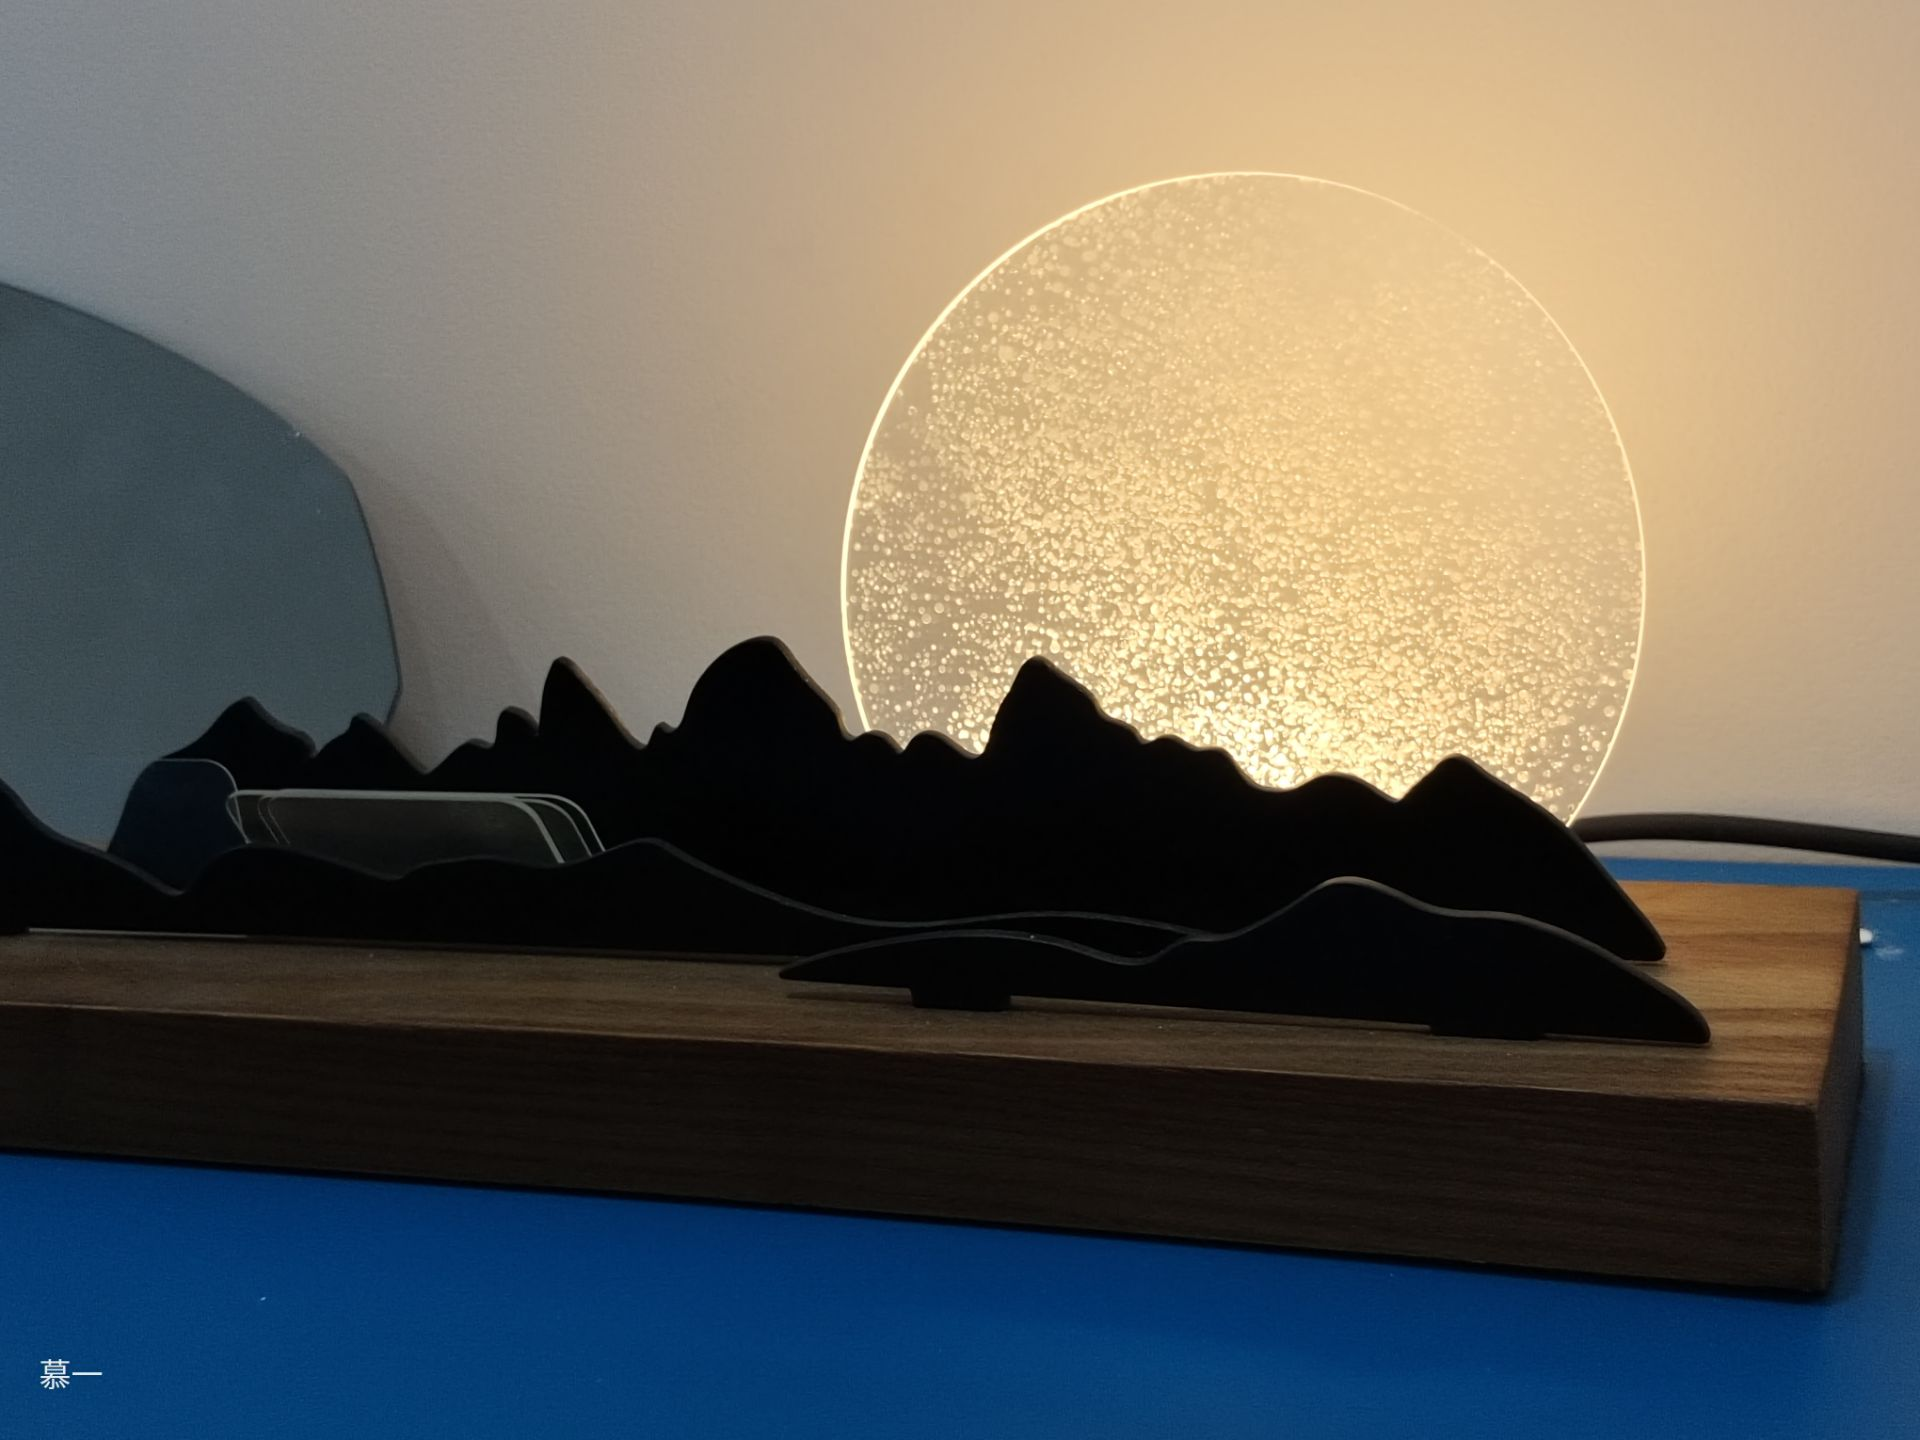
\includegraphics[width=0.45\textwidth]{1}}
		\subfigure{	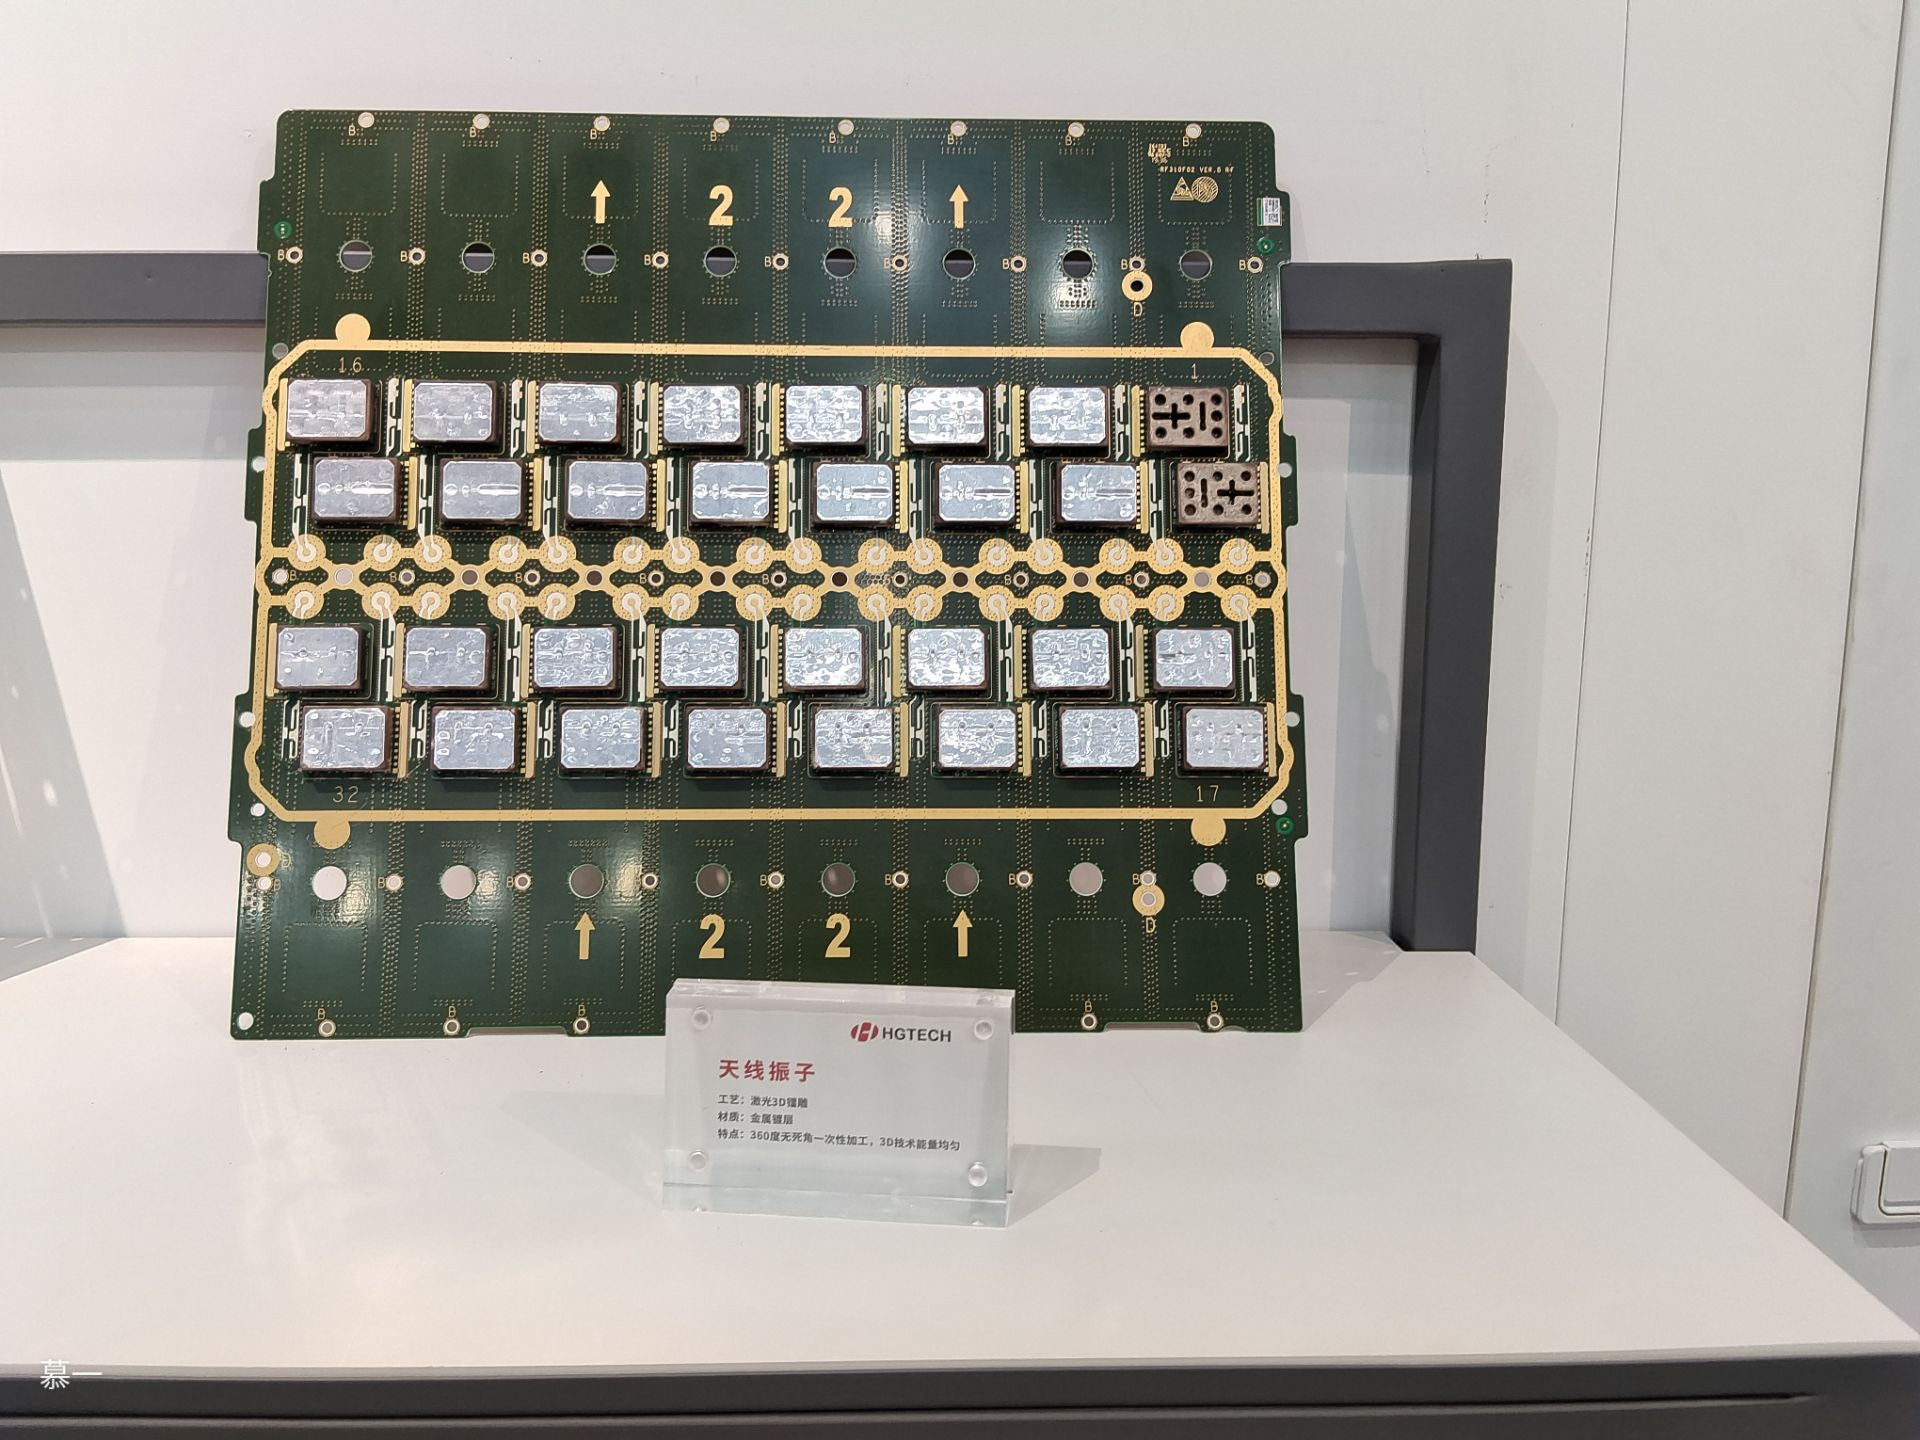
\includegraphics[width=0.45\textwidth]{2}}
\end{figure}
\end{document}

















